\documentclass[10pt]{article}
\usepackage{tikz}
\usetikzlibrary{shapes.misc}
\usepackage[margin=0cm]{geometry}
\pagestyle{empty}
\tikzstyle{every node}=[cross out, draw, red]

\begin{document}

\vspace*{\fill}
\begin{center}
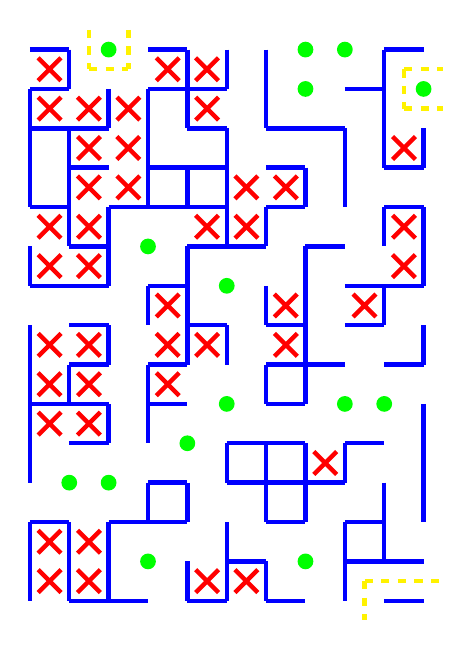
\begin{tikzpicture}[x=0.5cm, y=-0.5cm, ultra thick, blue]
% Walls
    \draw (0,0) -- (1,0);
    \draw (3,0) -- (4,0);
    \draw (9,0) -- (10,0);
    \draw (0,1) -- (1,1);
    \draw (3,1) -- (5,1);
    \draw (8,1) -- (9,1);
    \draw (0,2) -- (2,2);
    \draw (4,2) -- (5,2);
    \draw (6,2) -- (8,2);
    \draw (1,3) -- (2,3);
    \draw (3,3) -- (5,3);
    \draw (6,3) -- (7,3);
    \draw (9,3) -- (10,3);
    \draw (0,4) -- (1,4);
    \draw (2,4) -- (5,4);
    \draw (6,4) -- (7,4);
    \draw (9,4) -- (10,4);
    \draw (1,5) -- (2,5);
    \draw (4,5) -- (6,5);
    \draw (7,5) -- (8,5);
    \draw (0,6) -- (2,6);
    \draw (3,6) -- (4,6);
    \draw (8,6) -- (10,6);
    \draw (1,7) -- (2,7);
    \draw (4,7) -- (5,7);
    \draw (6,7) -- (7,7);
    \draw (8,7) -- (9,7);
    \draw (1,8) -- (2,8);
    \draw (3,8) -- (4,8);
    \draw (6,8) -- (8,8);
    \draw (9,8) -- (10,8);
    \draw (0,9) -- (2,9);
    \draw (3,9) -- (4,9);
    \draw (6,9) -- (7,9);
    \draw (1,10) -- (2,10);
    \draw (5,10) -- (7,10);
    \draw (8,10) -- (9,10);
    \draw (3,11) -- (4,11);
    \draw (5,11) -- (8,11);
    \draw (0,12) -- (1,12);
    \draw (2,12) -- (4,12);
    \draw (6,12) -- (7,12);
    \draw (8,12) -- (9,12);
    \draw (5,13) -- (6,13);
    \draw (8,13) -- (10,13);
    \draw (1,14) -- (3,14);
    \draw (4,14) -- (5,14);
    \draw (6,14) -- (7,14);
    \draw (9,14) -- (10,14);
    \draw (0,1) -- (0,4);
    \draw (0,5) -- (0,6);
    \draw (0,7) -- (0,11);
    \draw (0,12) -- (0,14);
    \draw (1,0) -- (1,1);
    \draw (1,2) -- (1,5);
    \draw (1,8) -- (1,9);
    \draw (1,12) -- (1,14);
    \draw (2,1) -- (2,2);
    \draw (2,4) -- (2,6);
    \draw (2,7) -- (2,8);
    \draw (2,9) -- (2,10);
    \draw (2,12) -- (2,14);
    \draw (3,1) -- (3,4);
    \draw (3,6) -- (3,7);
    \draw (3,8) -- (3,10);
    \draw (3,11) -- (3,12);
    \draw (4,0) -- (4,2);
    \draw (4,3) -- (4,4);
    \draw (4,5) -- (4,8);
    \draw (4,11) -- (4,12);
    \draw (4,13) -- (4,14);
    \draw (5,0) -- (5,1);
    \draw (5,2) -- (5,5);
    \draw (5,7) -- (5,8);
    \draw (5,10) -- (5,11);
    \draw (5,12) -- (5,14);
    \draw (6,0) -- (6,2);
    \draw (6,4) -- (6,5);
    \draw (6,6) -- (6,7);
    \draw (6,8) -- (6,9);
    \draw (6,10) -- (6,12);
    \draw (6,13) -- (6,14);
    \draw (7,3) -- (7,4);
    \draw (7,5) -- (7,9);
    \draw (7,10) -- (7,12);
    \draw (8,2) -- (8,4);
    \draw (8,10) -- (8,11);
    \draw (8,12) -- (8,14);
    \draw (9,0) -- (9,3);
    \draw (9,4) -- (9,5);
    \draw (9,6) -- (9,7);
    \draw (9,11) -- (9,13);
    \draw (10,2) -- (10,3);
    \draw (10,4) -- (10,6);
    \draw (10,7) -- (10,8);
    \draw (10,9) -- (10,12);
% Pillars
    \fill[green] (2,0) circle(0.2);
    \fill[green] (7,0) circle(0.2);
    \fill[green] (8,0) circle(0.2);
    \fill[green] (7,1) circle(0.2);
    \fill[green] (10,1) circle(0.2);
    \fill[green] (3,5) circle(0.2);
    \fill[green] (5,6) circle(0.2);
    \fill[green] (5,9) circle(0.2);
    \fill[green] (8,9) circle(0.2);
    \fill[green] (9,9) circle(0.2);
    \fill[green] (4,10) circle(0.2);
    \fill[green] (1,11) circle(0.2);
    \fill[green] (2,11) circle(0.2);
    \fill[green] (3,13) circle(0.2);
    \fill[green] (7,13) circle(0.2);
% Inner points in accessible cul-de-sacs
    \node at (0.5,0.5) {};
    \node at (3.5,0.5) {};
    \node at (4.5,0.5) {};
    \node at (0.5,1.5) {};
    \node at (1.5,1.5) {};
    \node at (2.5,1.5) {};
    \node at (4.5,1.5) {};
    \node at (1.5,2.5) {};
    \node at (2.5,2.5) {};
    \node at (9.5,2.5) {};
    \node at (1.5,3.5) {};
    \node at (2.5,3.5) {};
    \node at (5.5,3.5) {};
    \node at (6.5,3.5) {};
    \node at (0.5,4.5) {};
    \node at (1.5,4.5) {};
    \node at (4.5,4.5) {};
    \node at (5.5,4.5) {};
    \node at (9.5,4.5) {};
    \node at (0.5,5.5) {};
    \node at (1.5,5.5) {};
    \node at (9.5,5.5) {};
    \node at (3.5,6.5) {};
    \node at (6.5,6.5) {};
    \node at (8.5,6.5) {};
    \node at (0.5,7.5) {};
    \node at (1.5,7.5) {};
    \node at (3.5,7.5) {};
    \node at (4.5,7.5) {};
    \node at (6.5,7.5) {};
    \node at (0.5,8.5) {};
    \node at (1.5,8.5) {};
    \node at (3.5,8.5) {};
    \node at (0.5,9.5) {};
    \node at (1.5,9.5) {};
    \node at (7.5,10.5) {};
    \node at (0.5,12.5) {};
    \node at (1.5,12.5) {};
    \node at (0.5,13.5) {};
    \node at (1.5,13.5) {};
    \node at (4.5,13.5) {};
    \node at (5.5,13.5) {};
% Entry-exit paths without intersections
    \draw[dashed, yellow] (1.5,0.5) -- (2.5,0.5);
    \draw[dashed, yellow] (9.5,0.5) -- (10.5,0.5);
    \draw[dashed, yellow] (9.5,1.5) -- (10.5,1.5);
    \draw[dashed, yellow] (8.5,13.5) -- (10.5,13.5);
    \draw[dashed, yellow] (1.5,-0.5) -- (1.5,0.5);
    \draw[dashed, yellow] (2.5,-0.5) -- (2.5,0.5);
    \draw[dashed, yellow] (8.5,13.5) -- (8.5,14.5);
    \draw[dashed, yellow] (9.5,0.5) -- (9.5,1.5);
\end{tikzpicture}
\end{center}
\vspace*{\fill}

\end{document}
